% ============================================================
% HAT: Learning What to Learn for Self-Improving Language Models
% Target venue: NeurIPS 2026 (Main Track)
% Uses the official neurips_2026.sty
% ============================================================
\documentclass{article}

% --- Track / submission mode ---------------------------------
% Options provided by neurips_2026.sty:
%   (default)  — Main Track, anonymous double-blind submission (line numbers ON)
%   [main]     — Main Track (equivalent to default)
%   [preprint] — non-anonymous preprint (e.g., arXiv)
%   [final]    — camera-ready (de-anonymised, no line numbers)
%   [nonatbib] — disable automatic natbib loading
%
% At submission time, omit `final` and `preprint` to keep it anonymous.
\usepackage{neurips_2026}
% \usepackage[preprint]{neurips_2026}
% \usepackage[main, final]{neurips_2026}

% --- Standard packages (per official template) ---------------
\usepackage[utf8]{inputenc}
\usepackage[T1]{fontenc}
\usepackage{hyperref}
\usepackage{url}
\usepackage{booktabs}
\usepackage{amsfonts}
\usepackage{amsmath,amssymb}
\usepackage{nicefrac}
\usepackage{microtype}
\usepackage{xcolor}

% --- Additional packages used by the HAT paper ---------------
\usepackage{graphicx}
\usepackage{multirow}
\usepackage{enumitem}
\usepackage{bbm}
\usepackage{bm}
\usepackage{xspace}
\usepackage[ruled,vlined,linesnumbered]{algorithm2e}
\usepackage{tikz}
\usetikzlibrary{arrows.meta,positioning,fit,calc,backgrounds,shapes.geometric,shadows.blur}
\usepackage{fontawesome5}

% --- Custom math macros --------------------------------------
% math_commands.tex — Custom notation and macros for the HAT paper.
% Include via % math_commands.tex — Custom notation and macros for the HAT paper.
% Include via % math_commands.tex — Custom notation and macros for the HAT paper.
% Include via \input{math_commands} in the preamble.

% ===== General Math =====
\newcommand{\R}{\mathbb{R}}
\newcommand{\N}{\mathbb{N}}
\newcommand{\E}{\mathbb{E}}
\newcommand{\Var}{\mathrm{Var}}

% Probability / Expectation
\newcommand{\prob}[1]{\Pr\!\left(#1\right)}
\newcommand{\expect}[1]{\E\!\left[#1\right]}
\newcommand{\KL}[2]{\mathrm{KL}\!\left(#1 \,\Vert\, #2\right)}

% ===== Model Components =====
\newcommand{\model}{\mathcal{M}}                    % base model
\newcommand{\modeltheta}{\mathcal{M}_{\theta}}      % parameterised model
\newcommand{\cortex}{\mathcal{C}}                    % cortex module
\newcommand{\hippocampus}{\mathcal{H}}               % hippocampus agent
\newcommand{\oracle}{\mathcal{O}}                    % oracle / teacher LLM
\newcommand{\neocortex}{\mathcal{N}}                 % neocortex memory store
\newcommand{\sws}{\mathcal{SWS}}                     % slow-wave sleep trainer
\newcommand{\replaybuf}{\mathcal{B}}                 % replay buffer

% ===== Parameters =====
\newcommand{\params}{\theta}                         % model parameters
\newcommand{\paramsnew}{\theta^{\mathrm{new}}}       % updated parameters
\newcommand{\paramsold}{\theta_{\mathrm{old}}}       % previous parameters

% ===== Loss Functions =====
\newcommand{\loss}{\mathcal{L}}                      % generic loss
\newcommand{\lossce}{\mathcal{L}_{\mathrm{CE}}}     % cross-entropy loss
\newcommand{\losskd}{\mathcal{L}_{\mathrm{KD}}}     % knowledge distillation loss
\newcommand{\lossreg}{\mathcal{L}_{\mathrm{reg}}}   % regularisation loss
\newcommand{\losssws}{\mathcal{L}_{\mathrm{SWS}}}   % SWS trainer loss (combined)

% ===== Memory / Selection =====
\newcommand{\memtrace}{m}                             % memory trace
\newcommand{\memory}{\mathcal{M}}                     % memory collection
\newcommand{\metadata}{\xi}                           % trace metadata
\newcommand{\writepolicy}{\pi_{\mathrm{write}}}       % write policy
\newcommand{\selectscore}{s}                          % composite selection score
\newcommand{\uncertainty}{U}                          % uncertainty score
\newcommand{\feedback}{F}                             % feedback signal
\newcommand{\novelty}{N}                              % novelty score

% ===== Sequences / Tokens =====
\newcommand{\vocab}{\mathcal{V}}                     % vocabulary
\newcommand{\context}{c}                             % context
\newcommand{\seq}{x}                                 % input sequence
\newcommand{\seqy}{y}                                % output / target sequence
\newcommand{\query}{q}                               % user query
\newcommand{\response}{a}                            % model response

% ===== Miscellaneous =====
\newcommand{\ie}{\textit{i.e.}}
\newcommand{\eg}{\textit{e.g.}}
\newcommand{\cf}{\textit{cf.}}
\newcommand{\etal}{\textit{et~al.}}
\newcommand{\wrt}{w.r.t.\@\xspace}
\newcommand{\HAT}{\textsc{HAT}}                      % formatted model name

% ===== Operators =====
\DeclareMathOperator*{\argmax}{arg\,max}
\DeclareMathOperator*{\argmin}{arg\,min}
\DeclareMathOperator{\softmax}{softmax}
\DeclareMathOperator{\entropy}{H}
\newcommand{\cosine}{\mathrm{cos}}
\newcommand{\TopK}{\mathrm{TopK}}
\newcommand{\Merge}{\mathrm{Merge}}
\newcommand{\indicator}{\mathbbm{1}}
 in the preamble.

% ===== General Math =====
\newcommand{\R}{\mathbb{R}}
\newcommand{\N}{\mathbb{N}}
\newcommand{\E}{\mathbb{E}}
\newcommand{\Var}{\mathrm{Var}}

% Probability / Expectation
\newcommand{\prob}[1]{\Pr\!\left(#1\right)}
\newcommand{\expect}[1]{\E\!\left[#1\right]}
\newcommand{\KL}[2]{\mathrm{KL}\!\left(#1 \,\Vert\, #2\right)}

% ===== Model Components =====
\newcommand{\model}{\mathcal{M}}                    % base model
\newcommand{\modeltheta}{\mathcal{M}_{\theta}}      % parameterised model
\newcommand{\cortex}{\mathcal{C}}                    % cortex module
\newcommand{\hippocampus}{\mathcal{H}}               % hippocampus agent
\newcommand{\oracle}{\mathcal{O}}                    % oracle / teacher LLM
\newcommand{\neocortex}{\mathcal{N}}                 % neocortex memory store
\newcommand{\sws}{\mathcal{SWS}}                     % slow-wave sleep trainer
\newcommand{\replaybuf}{\mathcal{B}}                 % replay buffer

% ===== Parameters =====
\newcommand{\params}{\theta}                         % model parameters
\newcommand{\paramsnew}{\theta^{\mathrm{new}}}       % updated parameters
\newcommand{\paramsold}{\theta_{\mathrm{old}}}       % previous parameters

% ===== Loss Functions =====
\newcommand{\loss}{\mathcal{L}}                      % generic loss
\newcommand{\lossce}{\mathcal{L}_{\mathrm{CE}}}     % cross-entropy loss
\newcommand{\losskd}{\mathcal{L}_{\mathrm{KD}}}     % knowledge distillation loss
\newcommand{\lossreg}{\mathcal{L}_{\mathrm{reg}}}   % regularisation loss
\newcommand{\losssws}{\mathcal{L}_{\mathrm{SWS}}}   % SWS trainer loss (combined)

% ===== Memory / Selection =====
\newcommand{\memtrace}{m}                             % memory trace
\newcommand{\memory}{\mathcal{M}}                     % memory collection
\newcommand{\metadata}{\xi}                           % trace metadata
\newcommand{\writepolicy}{\pi_{\mathrm{write}}}       % write policy
\newcommand{\selectscore}{s}                          % composite selection score
\newcommand{\uncertainty}{U}                          % uncertainty score
\newcommand{\feedback}{F}                             % feedback signal
\newcommand{\novelty}{N}                              % novelty score

% ===== Sequences / Tokens =====
\newcommand{\vocab}{\mathcal{V}}                     % vocabulary
\newcommand{\context}{c}                             % context
\newcommand{\seq}{x}                                 % input sequence
\newcommand{\seqy}{y}                                % output / target sequence
\newcommand{\query}{q}                               % user query
\newcommand{\response}{a}                            % model response

% ===== Miscellaneous =====
\newcommand{\ie}{\textit{i.e.}}
\newcommand{\eg}{\textit{e.g.}}
\newcommand{\cf}{\textit{cf.}}
\newcommand{\etal}{\textit{et~al.}}
\newcommand{\wrt}{w.r.t.\@\xspace}
\newcommand{\HAT}{\textsc{HAT}}                      % formatted model name

% ===== Operators =====
\DeclareMathOperator*{\argmax}{arg\,max}
\DeclareMathOperator*{\argmin}{arg\,min}
\DeclareMathOperator{\softmax}{softmax}
\DeclareMathOperator{\entropy}{H}
\newcommand{\cosine}{\mathrm{cos}}
\newcommand{\TopK}{\mathrm{TopK}}
\newcommand{\Merge}{\mathrm{Merge}}
\newcommand{\indicator}{\mathbbm{1}}
 in the preamble.

% ===== General Math =====
\newcommand{\R}{\mathbb{R}}
\newcommand{\N}{\mathbb{N}}
\newcommand{\E}{\mathbb{E}}
\newcommand{\Var}{\mathrm{Var}}

% Probability / Expectation
\newcommand{\prob}[1]{\Pr\!\left(#1\right)}
\newcommand{\expect}[1]{\E\!\left[#1\right]}
\newcommand{\KL}[2]{\mathrm{KL}\!\left(#1 \,\Vert\, #2\right)}

% ===== Model Components =====
\newcommand{\model}{\mathcal{M}}                    % base model
\newcommand{\modeltheta}{\mathcal{M}_{\theta}}      % parameterised model
\newcommand{\cortex}{\mathcal{C}}                    % cortex module
\newcommand{\hippocampus}{\mathcal{H}}               % hippocampus agent
\newcommand{\oracle}{\mathcal{O}}                    % oracle / teacher LLM
\newcommand{\neocortex}{\mathcal{N}}                 % neocortex memory store
\newcommand{\sws}{\mathcal{SWS}}                     % slow-wave sleep trainer
\newcommand{\replaybuf}{\mathcal{B}}                 % replay buffer

% ===== Parameters =====
\newcommand{\params}{\theta}                         % model parameters
\newcommand{\paramsnew}{\theta^{\mathrm{new}}}       % updated parameters
\newcommand{\paramsold}{\theta_{\mathrm{old}}}       % previous parameters

% ===== Loss Functions =====
\newcommand{\loss}{\mathcal{L}}                      % generic loss
\newcommand{\lossce}{\mathcal{L}_{\mathrm{CE}}}     % cross-entropy loss
\newcommand{\losskd}{\mathcal{L}_{\mathrm{KD}}}     % knowledge distillation loss
\newcommand{\lossreg}{\mathcal{L}_{\mathrm{reg}}}   % regularisation loss
\newcommand{\losssws}{\mathcal{L}_{\mathrm{SWS}}}   % SWS trainer loss (combined)

% ===== Memory / Selection =====
\newcommand{\memtrace}{m}                             % memory trace
\newcommand{\memory}{\mathcal{M}}                     % memory collection
\newcommand{\metadata}{\xi}                           % trace metadata
\newcommand{\writepolicy}{\pi_{\mathrm{write}}}       % write policy
\newcommand{\selectscore}{s}                          % composite selection score
\newcommand{\uncertainty}{U}                          % uncertainty score
\newcommand{\feedback}{F}                             % feedback signal
\newcommand{\novelty}{N}                              % novelty score

% ===== Sequences / Tokens =====
\newcommand{\vocab}{\mathcal{V}}                     % vocabulary
\newcommand{\context}{c}                             % context
\newcommand{\seq}{x}                                 % input sequence
\newcommand{\seqy}{y}                                % output / target sequence
\newcommand{\query}{q}                               % user query
\newcommand{\response}{a}                            % model response

% ===== Miscellaneous =====
\newcommand{\ie}{\textit{i.e.}}
\newcommand{\eg}{\textit{e.g.}}
\newcommand{\cf}{\textit{cf.}}
\newcommand{\etal}{\textit{et~al.}}
\newcommand{\wrt}{w.r.t.\@\xspace}
\newcommand{\HAT}{\textsc{HAT}}                      % formatted model name

% ===== Operators =====
\DeclareMathOperator*{\argmax}{arg\,max}
\DeclareMathOperator*{\argmin}{arg\,min}
\DeclareMathOperator{\softmax}{softmax}
\DeclareMathOperator{\entropy}{H}
\newcommand{\cosine}{\mathrm{cos}}
\newcommand{\TopK}{\mathrm{TopK}}
\newcommand{\Merge}{\mathrm{Merge}}
\newcommand{\indicator}{\mathbbm{1}}


% --- Theorem environments ------------------------------------
\newtheorem{theorem}{Theorem}
\newtheorem{proposition}[theorem]{Proposition}
\newtheorem{lemma}[theorem]{Lemma}
\newtheorem{corollary}[theorem]{Corollary}
\newtheorem{definition}[theorem]{Definition}
\newtheorem{remark}[theorem]{Remark}

% ============================================================
%                      TITLE & AUTHORS
% ============================================================
% \title{Learning What to Learn for Self-Improving Language Models}
% \title{Learning What to Learn for Self-Adaptive Language Models}
% \title{HAT: Hippocampus-Augmented Transformer for Selective Memory Consolidation in Continual Learning}
% \title{Learning What to Learn: Selective Memory Consolidation for Continual Learning Model}
% \title{Selective Memory Consolidation for Continual Learning Model}
% \title{Learning What to Learn: Memory-Selective Continual Adaptation for Language Models}
\title{Learning What to Learn: Hippocampal Memory Consolidation for Continual Model Adaptation}

% Authors are automatically anonymised in submission mode by the style file.
% For [preprint] or [final], replace with real names/affiliations.
\author{%
  Anonymous Author(s) \\
  Affiliation \\
  Address \\
  \texttt{email}
  % Example with multiple authors:
  % First Author\thanks{Equal contribution.} \\
  % Department of Computer Science \\
  % University \\
  % \texttt{first@example.com} \\
  % \And
  % Second Author \\
  % Affiliation \\
  % Address \\
  % \texttt{second@example.com} \\
}

\begin{document}

\maketitle

% ============================================================
%                         ABSTRACT
% ============================================================
% \begin{abstract}
% Contemporary large language models are pre-trained on internet-scale, broadly sourced text corpora and scale to hundreds of billions of parameters, incurring substantial training and deployment costs, while relying on expensive and iterative post hoc adaptation for downstream alignment.
% Human cognition, by contrast, is selective and experience-driven, relying on hippocampal mechanisms that preferentially encode salient, novel, or behaviorally relevant experiences for long-term consolidation.
% We propose \textbf{HAT (Hippocampus-Augmented Transformer)}, a memory-centric self-improvement paradigm that enables language models to learn \emph{what to learn} from experience.
% Inspired by hippocampal and neocortical memory consolidation in the mammalian brain, HAT introduces a mechanism of \emph{selective memory consolidation} that transforms raw user interactions into structured, high-fidelity training signals through three stages of abstraction, selection, and replay.
% Rather than indiscriminately storing data, HAT prioritises high-value experiences based on model uncertainty, explicit user feedback, and input novelty, and converts them into reusable learning signals.
% HAT operates in a wake and sleep loop.
% During online interaction, the base language model, which we term the \emph{Cortex}, estimates its own uncertainty and selectively incorporates user corrections or consults an external oracle, namely a stronger teacher model.
% During offline \emph{slow-wave sleep} (SWS) phases, curated experiences stored in a \emph{Neocortex} memory are replayed to update model parameters via targeted fine-tuning.
% This decoupling of experience acquisition from parameter optimisation enables stable and sample-efficient continual learning without catastrophic forgetting.
% We evaluate HAT on knowledge-intensive question answering, instruction following, and personalisation benchmarks.
% Experimental results demonstrate that HAT consistently outperforms strong fine-tuning and retrieval-augmented baselines, achieving significant gains in sample efficiency, error-rate reduction, and long-horizon adaptation, validating the effectiveness of learning through selective memory consolidation.
% \end{abstract}

% \begin{abstract}
% Contemporary language models are trained on internet-scale corpora and scaled to hundreds of billions of parameters, incurring substantial costs in training, deployment and post hoc adaptation.
% Human cognition, by contrast, is selective and experience-driven, relying on hippocampal mechanisms that preferentially encode salient, novel, or behaviorally relevant experiences and coordinate their gradual consolidation into long-term neocortical memory.
% We propose \textbf{Hippocampus-Augmented Transformer (HAT)}, a memory-centric self-improvement approach inspired by hippocampal and neocortical memory consolidation in the mammalian brain.
% HAT enables small language models to learn \emph{what to learn} from interaction by modeling three core hippocampal functions: rapid abstraction of experience, selective retention of informative traces, and replay-based consolidation during offline sleep-like phases.
% During the wake phase, a base model, the \emph{Cortex}, serves user queries while a \emph{Hippocampus Agent} transforms interactions and corrections into structured memory traces, scores them using uncertainty, feedback, and novelty, and consults an external oracle when additional supervision is needed.
% Selected traces are written to a long-term \emph{Neocortex} memory and replayed during \emph{slow-wave sleep} (SWS) phases, where an SWS trainer updates the Cortex through parameter-efficient fine-tuning.
% This wake--sleep separation turns sparse feedback and uncertain interactions into reusable training signals while limiting indiscriminate data accumulation.
% We evaluate HAT on knowledge-intensive question answering, instruction following, and personalization benchmarks, comparing it with fine-tuning and retrieval-augmented baselines under continual adaptation settings.
% \end{abstract}

\begin{abstract}
Contemporary language models are trained on internet-scale corpora and scaled to massive parameter regimes, incurring substantial costs in training, deployment, and continual adaptation.
Human cognition, by contrast, is selective and experience-driven, relying on hippocampal mechanisms that preferentially encode salient, novel, and behaviorally relevant experiences and coordinate their gradual consolidation into long-term neocortical memory.
We propose \textbf{Hippocampus-Augmented Transformer (HAT)}, a memory-centric continual learning mechanism inspired by hippocampal--neocortical consolidation in the mammalian brain.
HAT enables language models to learn \emph{what to learn} from interaction by coupling online experience acquisition with offline memory consolidation.
During interaction, a base model (the \emph{Cortex}) processes inputs while a \emph{Hippocampus Agent} encodes interactions and feedback into structured memory traces and selectively retains informative experiences based on uncertainty, novelty, and supervision signals, optionally querying an external oracle when needed.
Selected experiences are progressively consolidated into a persistent \emph{Neocortex} memory and subsequently replayed during slow-wave sleep (SWS), where the Cortex is updated through parameter-efficient fine-tuning.
This wake--sleep separation transforms sparse, interaction-driven feedback into reusable training signals, enabling continual self-improvement without indiscriminate data accumulation.
We evaluate HAT on knowledge-intensive question answering, instruction following, and personalization benchmarks, demonstrating consistent improvements over fine-tuning and retrieval-augmented baselines under continual adaptation settings.
\end{abstract}

% \begin{abstract}
% Contemporary language models are trained on internet-scale corpora and scaled to massive parameter regimes, incurring substantial costs in training, deployment, and continual adaptation.
% Human cognition, by contrast, is selective and experience-driven, relying on hippocampal mechanisms that preferentially encode salient, novel, and behaviorally relevant experiences and coordinate their gradual consolidation into long-term neocortical memory.
% We propose \textbf{Hippocampus-Augmented Transformer (HAT)}, a hippocampus-inspired continual learning mechanism that enables language models to learn \emph{what to learn} through selective memory consolidation.
% HAT separates wake-phase interaction from sleep-phase adaptation: during wake, a base model (the \emph{Cortex}) processes inputs while a \emph{Hippocampus Agent} encodes interactions and feedback into structured memory traces, selectively retaining experiences according to uncertainty, novelty, and supervision signals.
% When additional supervision is needed, the Hippocampus Agent queries an external oracle and integrates its response into the retained trace.
% Selected traces are progressively consolidated into a persistent \emph{Neocortex} memory and replayed during slow-wave sleep (SWS), where the Cortex is updated through parameter-efficient fine-tuning.
% This wake--sleep mechanism transforms sparse interaction feedback into reusable training signals, enabling continual self-improvement without indiscriminate data accumulation.
% We evaluate HAT on knowledge-intensive question answering, instruction following, and personalization benchmarks, demonstrating consistent improvements over fine-tuning and retrieval-augmented baselines under continual adaptation settings.
% \end{abstract}

% ============================================================
%                     MAIN BODY
% ============================================================
% ============================================================
% Section 1 — Introduction
% ============================================================
\section{Introduction}
\label{sec:introduction}

Large language models (LLMs) have demonstrated remarkable capabilities across a broad spectrum of natural language tasks~\citep{brown2020language,touvron2023llama,openai2023gpt4}.
Yet a fundamental tension remains: once training concludes, a model's knowledge is \emph{frozen}, and adapting it to new domains, user preferences, or corrected information requires costly retraining on carefully curated data.
This limitation is particularly acute for lightweight, on-device language models in the 0.5--10\,B parameter range, where users interact with a personal assistant that must evolve over time but lacks the infrastructure for large-scale retraining.

Existing approaches to post-deployment adaptation fall broadly into two categories.
\emph{Retrieval-augmented generation} (RAG) methods~\citep{lewis2020retrieval,guu2020realm} augment the model's context with external knowledge at inference time, but they do not update the model's parameters and thus cannot internalise corrections or new skills.
\emph{Continual fine-tuning} methods~\citep{kirkpatrick2017overcoming,de2021continual} update model weights on new data, but they typically require hand-curated datasets and are susceptible to catastrophic forgetting when data is noisy or unbalanced.
Neither paradigm addresses the upstream question: \emph{what should a model learn from?}

In biological intelligence, this problem is solved elegantly.
The mammalian hippocampus does not store all sensory experience; instead, it selectively encodes salient events and, during sleep, replays and consolidates them into long-term neocortical memory~\citep{mcclelland1995there,kumaran2016learning}.
This process of \emph{selective memory consolidation} ensures that only high-value experiences---those that are novel, surprising, or corrective---are used to update long-term knowledge.

Inspired by this principle, we propose \textbf{HAT (Hippocampus-Augmented Transformer)}, a multi-agent framework that equips a lightweight language model with the ability to \emph{learn what to learn} from its own interactions.
HAT introduces a dedicated \emph{Hippocampus Agent} that monitors the base model's (the \emph{Cortex}) interactions with users, abstracts raw dialogues into structured memory traces, selects high-value experiences using uncertainty, feedback, and novelty signals, and constructs training-ready replay data.
During offline phases---analogous to \emph{slow-wave sleep} (SWS) in the brain---curated experiences are replayed to fine-tune the Cortex, producing an improved model that re-enters the interaction loop.
When the Cortex is uncertain or produces errors, HAT can also consult an external \emph{Oracle} (a stronger teacher model), enabling a form of on-demand knowledge distillation.

\paragraph{Contributions.}
Our contributions are three-fold:
\begin{enumerate}[leftmargin=*,itemsep=2pt,topsep=3pt]
  \item We formalise the problem of \emph{selective experience curation} for self-improving language models and propose HAT, a memory-centric framework that decouples experience acquisition from parameter optimisation.
  \item We design a Hippocampus Agent with three composable stages---\emph{abstraction}, \emph{selection}, and \emph{replay construction}---that convert raw interactions into high-quality training signals using uncertainty estimation, user feedback, and novelty detection.
  \item We conduct extensive experiments on knowledge-intensive QA, instruction following, and personalisation benchmarks, demonstrating that HAT achieves consistent improvements in sample efficiency, error-rate reduction, and long-horizon adaptation over strong fine-tuning and retrieval-augmented baselines.
\end{enumerate}

% ============================================================
% Section 2 — Related Work
% ============================================================
\section{Related Work}
\label{sec:related_work}

\subsection{Continual Learning for Language Models}

Continual learning (CL) aims to update model parameters on a stream of tasks without catastrophic forgetting~\citep{kirkpatrick2017overcoming,zenke2017continual}.
Regularisation-based methods penalise changes to important weights~\citep{kirkpatrick2017overcoming,li2017learning}, while replay-based methods store or generate past examples for interleaved training~\citep{de2021continual,scialom2022fine}.
Recent work has extended CL to large language models, studying instruction tuning across sequential tasks~\citep{wu2024continual} and domain-incremental adaptation~\citep{ke2023continual}.
However, existing CL methods assume a \emph{given} data stream and do not address the problem of \emph{which} experiences should be retained.
HAT complements CL by introducing a principled experience selection mechanism upstream of parameter updates.

\subsection{Memory-Augmented Neural Networks}

Memory-augmented architectures equip neural networks with external memory stores that can be read from and written to~\citep{graves2014neural,sukhbaatar2015end}.
More recent work combines retrieval mechanisms with language models~\citep{borgeaud2022improving,zhong2022training}, enabling access to a large knowledge base at inference time.
While these approaches augment \emph{inference}, they do not leverage memory for \emph{learning}: retrieved information is used contextually but does not update the model's parameters.
In contrast, HAT uses its memory store (the Neocortex) as a curated training set that feeds back into parameter optimisation.

\subsection{Retrieval-Augmented Generation}

Retrieval-augmented generation (RAG) methods prepend retrieved passages to the model's input context~\citep{lewis2020retrieval,guu2020realm,izacard2022atlas}.
RAG is effective for knowledge-intensive tasks but inherits the limitations of fixed-context approaches: the model cannot \emph{learn} from retrieved content, context windows are bounded, and retrieval quality degrades when the knowledge base is noisy.
HAT can be seen as going beyond RAG by closing the loop from retrieval to training: high-value interactions—including oracle-provided corrections—are not only used at inference time but are consolidated into the model's parameters.

\subsection{Knowledge Distillation and Self-Improvement}

Knowledge distillation transfers knowledge from a teacher model to a student~\citep{hinton2015distilling,sanh2019distilbert}.
Recent work explores \emph{self-improving} language models that generate their own training data~\citep{huang2023large,yuan2024self,chen2024self} or use reinforcement learning from human/AI feedback~\citep{ouyang2022training,bai2022constitutional}.
These methods typically apply distillation or self-play uniformly, without selecting \emph{which} experiences are most informative.
HAT's Oracle consultation mechanism is a form of selective, on-demand distillation: the teacher is queried only when the student model is uncertain or has been corrected by the user, ensuring efficient use of the oracle's capacity.

\subsection{Complementary Learning Systems Theory}

Complementary learning systems (CLS) theory posits that the brain uses two interacting memory systems: the hippocampus for rapid encoding of specific episodes and the neocortex for slow extraction of statistical regularities~\citep{mcclelland1995there,kumaran2016learning}.
Sleep replay, particularly during slow-wave sleep, is hypothesised to mediate the transfer from hippocampus to neocortex~\citep{rasch2013sleep,walker2017sleep}.
Several works in machine learning have drawn on CLS for continual learning~\citep{shin2017continual,van2020brain,arani2022learning}, but they focus on image classification and do not address the unique challenges of language model self-improvement from interactive experience.
HAT directly operationalises the CLS framework for LLMs, with an explicit hippocampal selection stage, a neocortical memory store, and an offline SWS training phase.

% ============================================================
% Section 3 — Method
% ============================================================
\section{HAT: Hippocampus-Augmented Transformer}
\label{sec:method}

We present \textbf{Hippocampus-Augmented Transformer (HAT)}, a memory-centric continual learning approach that enables language models to learn \emph{what to learn} from interaction.
HAT is inspired by hippocampal--neocortical memory consolidation in the mammalian brain, where salient experiences are rapidly encoded, selectively retained, and later replayed for gradual integration into long-term cortical memory.
Rather than updating a model from all observed interactions, HAT separates online experience acquisition from offline model adaptation: during the \emph{wake phase}, interaction traces are selectively consolidated into a long-term memory; during the \emph{slow-wave sleep} (SWS) phase, selected traces are replayed as training signals to update the model.

As shown in Figure~\ref{fig:architecture}, HAT consists of four functional components.
The \textbf{Cortex} $\modeltheta$ is a lightweight language model that interacts with users.
The \textbf{Hippocampus Agent} $\hippocampus$ abstracts interactions into structured memory traces, estimates their learning value, and determines whether they should be retained.
The \textbf{Neocortex} $\neocortex$ is a persistent long-term memory that stores selected traces and their replay-ready training forms.
The \textbf{SWS Trainer} periodically updates the Cortex by replaying curated memories from the Neocortex.
An external \textbf{Oracle} $\oracle$ may be queried on demand when the Cortex is uncertain or when user feedback indicates an error.

\begin{figure}[t]
  \centering
  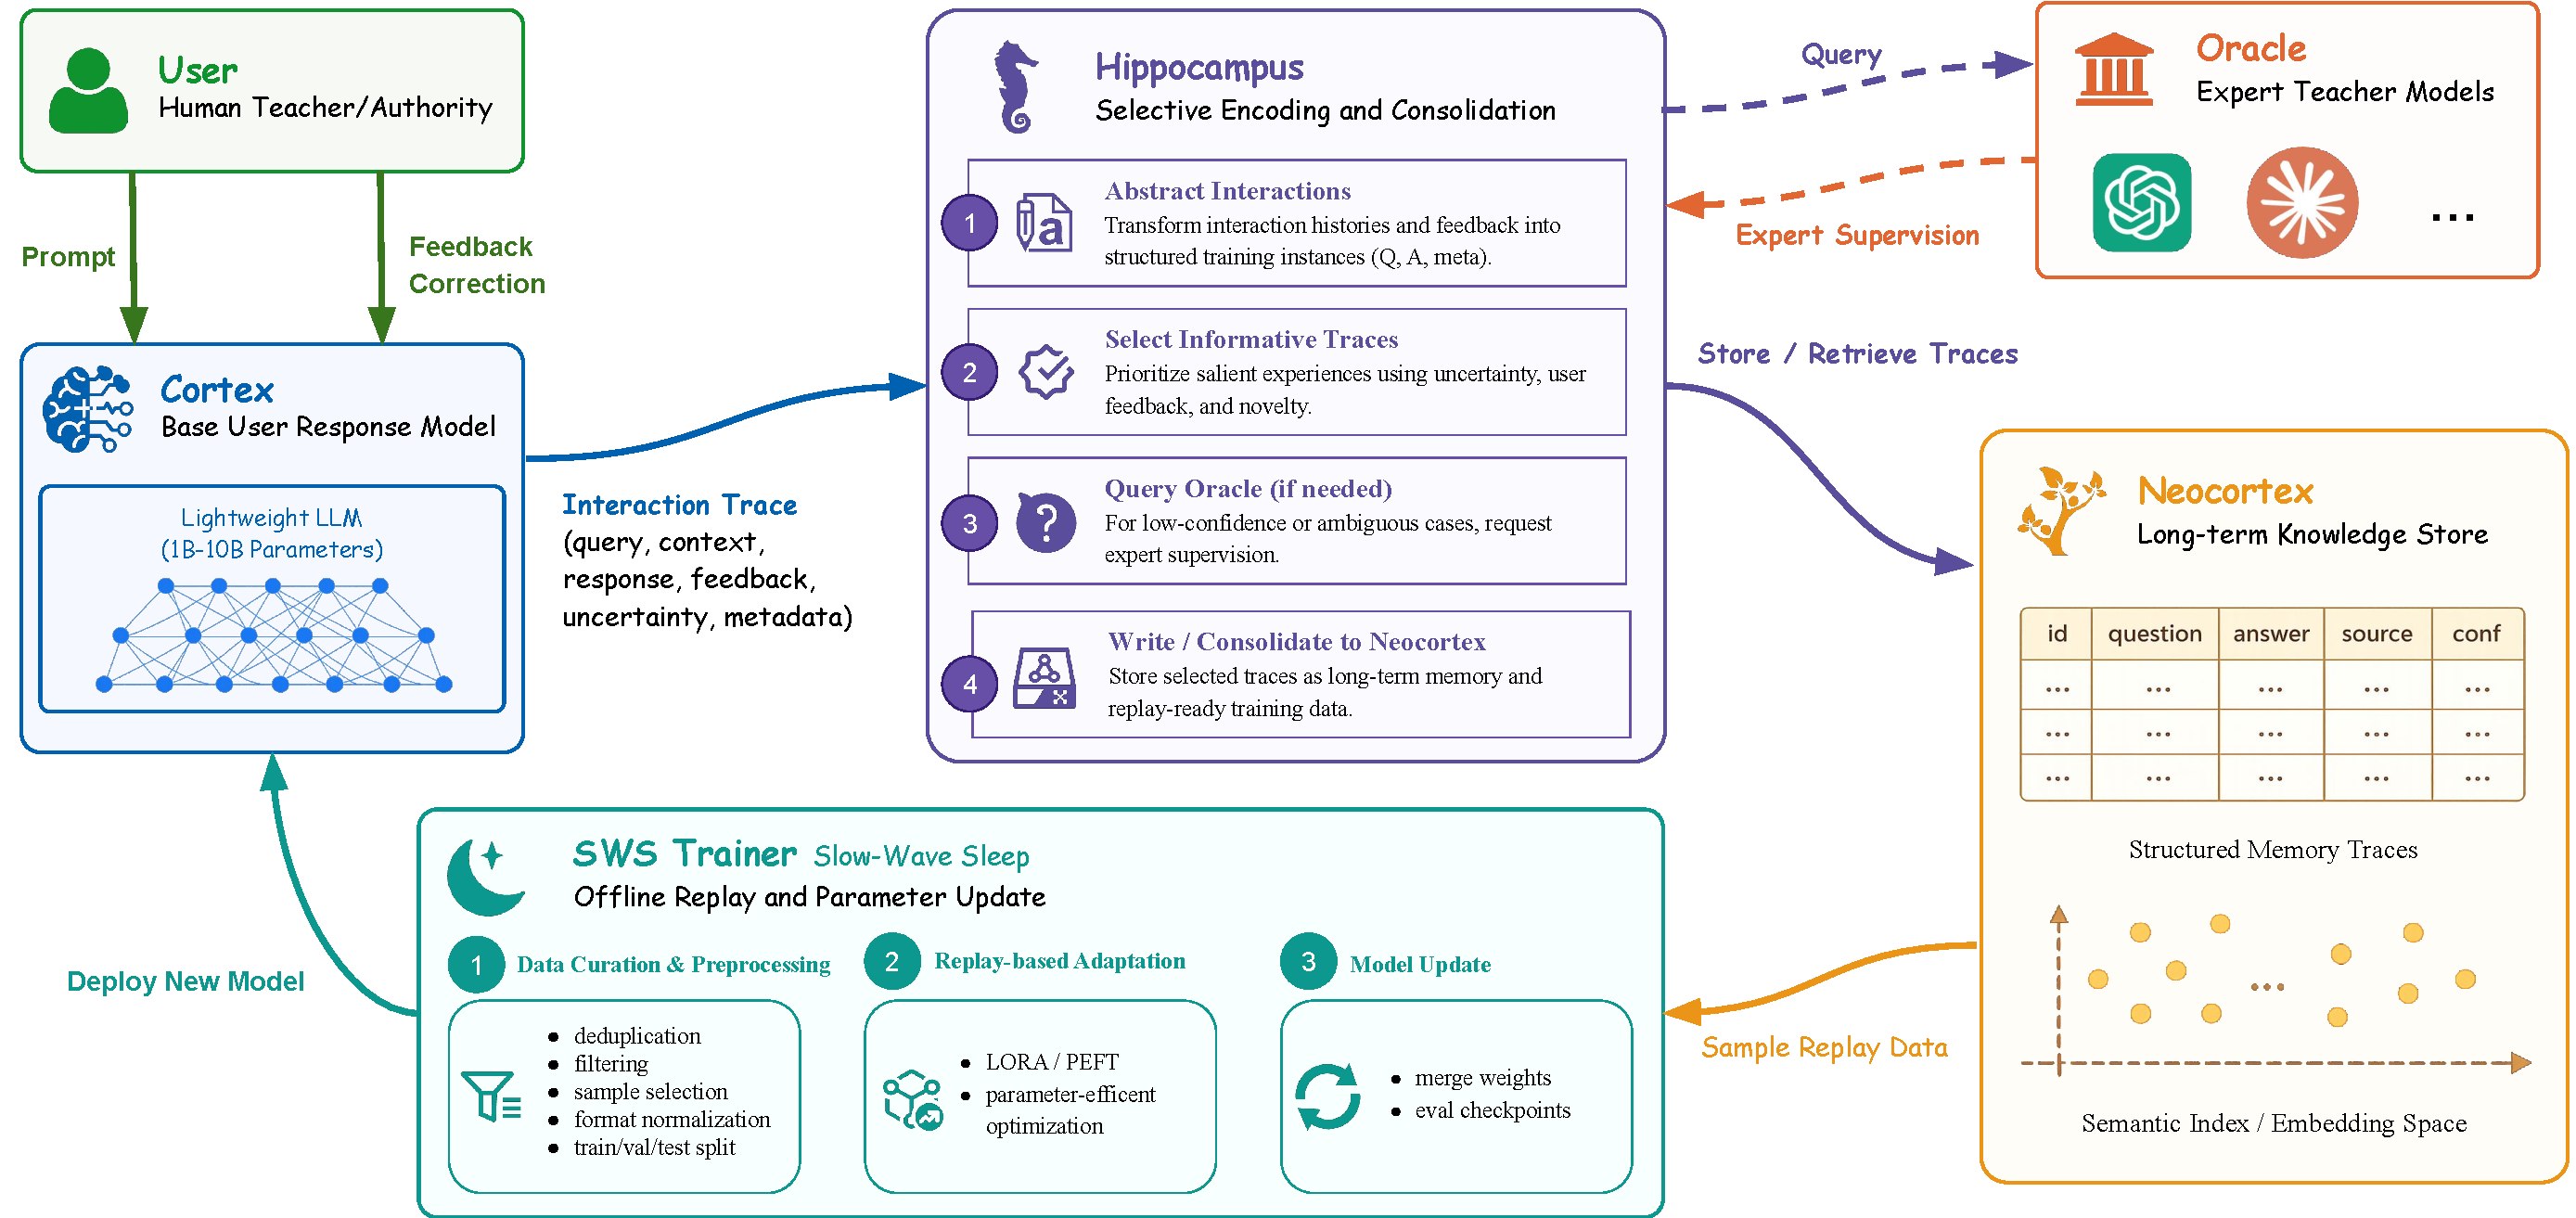
\includegraphics[width=\linewidth]{figures/framework.pdf}
  \caption{
    Overview of HAT, a hippocampus-inspired continual learning mechanism that converts selected interaction experiences into reusable training signals.
    During wake-phase interaction, the Cortex responds to user prompts while the Hippocampus encodes, selects, and optionally augments informative traces with Oracle supervision.
    The selected traces are consolidated into the Neocortex and replayed during slow-wave sleep (SWS), where the SWS Trainer updates the Cortex through parameter-efficient fine-tuning for continual self-improvement.
  }
  \label{fig:architecture}
\end{figure}

% ────────────────────────────────────────────────────────────
\subsection{Selective Learning Formulation}
\label{sec:method:formulation}

HAT treats continual adaptation as a selective learning problem over an interaction stream.
Let
\begin{equation}
  \mathcal{D}^{(t)} = \{x_i\}_{i=1}^{T_t}
\end{equation}
denote the set of interactions observed during wake cycle $t$, where each interaction is represented as
\begin{equation}
  x_i = (\context_i, \seq_i, \seqy_i, f_i),
\end{equation}
with context $\context_i$, user query $\seq_i$, model response $\seqy_i$, and optional feedback signal $f_i$.
The goal is not to learn from every interaction, but to identify a subset of experiences that are likely to improve the model under a limited adaptation budget.

Ideally, one would select experiences according to their expected learning gain:
\begin{equation}
  \mathcal{D}^{*(t)}
  =
  \arg\max_{\mathcal{D}' \subseteq \mathcal{D}^{(t)}}
  \;
  \mathbb{E}_{x \sim \mathcal{D}'}
  \left[
    \Delta \mathcal{L}(\params; x)
    \right],
  \label{eq:ideal_selection}
\end{equation}
where $\Delta \mathcal{L}(\params; x)$ denotes the expected reduction in future loss after adapting the model on experience $x$.
Since this quantity is generally unobservable at selection time, HAT approximates expected learning gain using observable proxies:
model uncertainty, external feedback, and semantic novelty.
This converts continual learning from indiscriminate data accumulation into a selective memory consolidation process.

% ────────────────────────────────────────────────────────────
\subsection{Wake--Sleep Learning Cycle}
\label{sec:method:wake_sleep}

HAT alternates between two complementary phases.

\paragraph{Wake phase.}
During the wake phase, the Cortex $\modeltheta$ receives a user query $\seq$ under context $\context$ and generates a response $\seqy$.
The resulting interaction is passed to the Hippocampus Agent, which compresses it into a memory trace, evaluates its utility, and determines whether it should be consolidated into the Neocortex.
If the Cortex is uncertain or the user provides corrective feedback, the Hippocampus Agent may consult the Oracle to obtain additional supervision.

\paragraph{Sleep phase.}
During the SWS phase, selected traces stored in the Neocortex are replayed as training examples.
The SWS Trainer updates the Cortex parameters using a curated replay distribution:
\begin{equation}
  \params^{(t+1)}
  =
  \mathrm{SWS}
  \left(
  \params^{(t)}, \neocortex^{(t)}
  \right).
  \label{eq:sws_transition}
\end{equation}
The updated model then becomes the Cortex for the next wake cycle.
Thus, HAT separates the decision of \emph{what should be learned} from the optimization process that performs the actual learning.

% ────────────────────────────────────────────────────────────
\subsection{Cortex: Online Interaction Model}
\label{sec:method:cortex}

The Cortex is an autoregressive Transformer language model $\modeltheta$ with parameters $\params$.
It can be instantiated by any lightweight model suitable for deployment, such as a model in the 0.5--10B parameter range.
Given context $\context$ and query $\seq$, the Cortex generates a response $\seqy = (y_1,\ldots,y_{|\seqy|})$ according to
\begin{equation}
  p_{\params}(\seqy \mid \context, \seq)
  =
  \prod_{j=1}^{|\seqy|}
  p_{\params}
  \left(
  y_j \mid \context, \seq, \seqy_{<j}
  \right).
  \label{eq:autoregressive}
\end{equation}

In addition to producing a response, the Cortex provides an uncertainty estimate $U(x)$ for each interaction.
In practice, $U(x)$ can be computed from predictive entropy, token-level confidence, self-consistency variance, or disagreement between sampled generations.
A simple entropy-based estimate is
\begin{equation}
  U(x)
  =
  \frac{1}{|\seqy|}
  \sum_{j=1}^{|\seqy|}
  H
  \left(
  p_{\params}
  (\cdot \mid \context, \seq, \seqy_{<j})
  \right),
  \label{eq:uncertainty}
\end{equation}
where $H(\cdot)$ denotes entropy.
High uncertainty indicates a potential epistemic gap and serves as one signal for selective memory consolidation.

% ────────────────────────────────────────────────────────────
\subsection{Hippocampus Agent: Selective Memory Consolidation}
\label{sec:method:hippocampus}

The Hippocampus Agent is the central mechanism of HAT.
It transforms raw interactions into structured memory traces and determines which traces should be consolidated into the Neocortex.
This process consists of three operations: abstraction, selection, and replay construction.

% --- 3.x.1 Abstraction ---
\subsubsection{Experience Abstraction}
\label{sec:method:abstraction}

Raw interaction logs are often verbose, redundant, and unsuitable for direct training.
The abstraction operation maps an interaction $x = (\context,\seq,\seqy,f)$ into a compact memory trace:
\begin{equation}
  \memtrace
  =
  \hippocampus_{\mathrm{abs}}
  (\context,\seq,\seqy,f).
  \label{eq:abstraction}
\end{equation}
The trace $\memtrace$ preserves the learning-relevant content of the episode, including the user intent, the model response, the corrected answer if available, and relevant contextual constraints.
This operation is analogous to rapid hippocampal encoding, where an experience is compressed into a retrievable trace rather than stored as an unfiltered sensory stream.

In implementation, $\hippocampus_{\mathrm{abs}}$ can be instantiated as a prompting procedure, a small summarization model, or the Cortex itself under an instruction template.
A memory trace may be represented as
\begin{equation}
  \memtrace
  =
  \left(
  q,\;
  a_{\mathrm{cortex}},\;
  a_{\mathrm{target}},\;
  r,\;
  \metadata
  \right),
  \label{eq:memory_trace}
\end{equation}
where $q$ is the normalized query, $a_{\mathrm{cortex}}$ is the Cortex response, $a_{\mathrm{target}}$ is the preferred target answer, $r$ is the rationale or correction signal, and $\metadata$ contains timestamp, source, uncertainty, feedback, and novelty statistics.

% --- 3.x.2 Selection ---
\subsubsection{Selection via Write Policy}
\label{sec:method:selection}

Not all traces should be stored or replayed.
HAT therefore defines a write policy $\writepolicy$ that estimates the consolidation value of each memory trace.
Given a trace $\memtrace$, the policy computes
\begin{equation}
  \mathrm{score}(\memtrace)
  =
  \alpha U(\memtrace)
  +
  \beta F(\memtrace)
  +
  \gamma N(\memtrace),
  \label{eq:selection_score}
\end{equation}
where $U$, $F$, and $N$ denote uncertainty, feedback, and novelty, respectively.

\paragraph{Uncertainty.}
$U(\memtrace)$ estimates the extent to which the Cortex is unreliable on the corresponding interaction.
High uncertainty suggests that the trace lies near the boundary of the model's current competence and may yield high learning value.

\paragraph{Feedback.}
$F(\memtrace)$ captures explicit or implicit supervision.
For example, user corrections, negative ratings, or contradiction signals can be mapped to a binary or graded value.
When an explicit correction is provided, $F(\memtrace)$ is assigned high priority to ensure that verified errors are consolidated.

\paragraph{Novelty.}
$N(\memtrace)$ measures the semantic distance between the current trace and the existing Neocortex memory.
Let $e(\memtrace)$ be an embedding of the trace and $\neocortex$ be the current memory store.
A practical novelty score is
\begin{equation}
  N(\memtrace)
  =
  1 -
  \max_{\memtrace' \in \neocortex}
  \cos
  \left(
  e(\memtrace), e(\memtrace')
  \right).
  \label{eq:novelty}
\end{equation}
Novel traces are prioritized because they expand coverage of underrepresented regions in the model's knowledge space.

The final write decision is
\begin{equation}
  z(\memtrace)
  =
  \mathbbm{1}
  \left[
    \mathrm{score}(\memtrace) > \tau
    \right],
  \label{eq:write_decision}
\end{equation}
where $\tau$ is a tunable consolidation threshold.
The coefficients $\alpha,\beta,\gamma$ control the relative importance of epistemic uncertainty, external supervision, and semantic coverage.

This write policy can be interpreted as a tractable surrogate for Equation~\ref{eq:ideal_selection}: uncertainty approximates knowledge gaps, feedback identifies externally verified errors, and novelty encourages memory diversity.

% --- 3.x.3 Replay Construction ---
\subsubsection{Replay Construction}
\label{sec:method:replay}

Selected memory traces must be converted into training-ready signals.
For each retained trace $\memtrace$, the Replay Builder produces one or more supervised examples:
\begin{equation}
  (\seq^{\mathrm{train}}, \seqy^{\mathrm{train}})
  \sim
  p_{\mathrm{replay}}(\cdot \mid \memtrace)
  =
  \hippocampus_{\mathrm{replay}}(\memtrace).
  \label{eq:replay_distribution}
\end{equation}
The replay distribution can include direct instruction--response pairs, corrected QA pairs, rationale-augmented examples, or contrastive pairs that distinguish the original erroneous response from the preferred target.

This step is important because memory consolidation in HAT is not merely storage.
A retained trace becomes useful only when it is transformed into a form that can drive gradient-based learning.
Thus, the Hippocampus Agent converts interaction experience into reusable training signals.

% ────────────────────────────────────────────────────────────
\subsection{Oracle: On-Demand External Supervision}
\label{sec:method:oracle}

The Oracle $\oracle$ is an external teacher used only when additional supervision is expected to be valuable.
Rather than distilling a large teacher model over an entire corpus, HAT queries the Oracle selectively.
The Oracle is invoked when the uncertainty exceeds a threshold $\tau_{\oracle}$ or when user feedback indicates an error:
\begin{equation}
  \seqy^{\oracle}
  =
  \oracle(\context,\seq),
  \quad
  \text{if }
  U(x) > \tau_{\oracle}
  \text{ or }
  F(x) > 0.
  \label{eq:oracle_query}
\end{equation}

The Oracle response may replace, refine, or supplement the Cortex response in the memory trace:
\begin{equation}
  a_{\mathrm{target}}
  =
  \mathrm{Merge}
  \left(
  a_{\mathrm{cortex}},
  a_{\mathrm{user}},
  a_{\oracle}
  \right),
  \label{eq:oracle_merge}
\end{equation}
where $a_{\mathrm{user}}$ denotes a user-provided correction when available.
This mechanism implements budget-aware supervision: teacher knowledge is acquired primarily at the frontier of the student's uncertainty or error, where it is most likely to improve future behavior.

% ────────────────────────────────────────────────────────────
\subsection{Neocortex: Long-Term Memory Store}
\label{sec:method:neocortex}

The Neocortex $\neocortex$ is a persistent memory store containing selected traces and their replay-ready training forms.
At wake cycle $t$, the memory is updated as
\begin{equation}
  \neocortex^{(t)}
  =
  \neocortex^{(t-1)}
  \cup
  \left\{
  \memtrace_i
  \;:\;
  z(\memtrace_i)=1
  \right\}.
  \label{eq:neocortex_update}
\end{equation}

Each memory entry stores both semantic content and training metadata:
\begin{equation}
  \neocortex
  =
  \left\{
  \left(
  \memtrace_i,\;
  \mathcal{R}_i,\;
  \mathrm{score}_i,\;
  \metadata_i
  \right)
  \right\}_{i=1}^{|\neocortex|},
  \label{eq:neocortex_structure}
\end{equation}
where $\mathcal{R}_i$ denotes replay examples generated from trace $\memtrace_i$.
In implementation, the Neocortex can be realized as a vector-indexed datastore with structured fields, allowing retrieval, deduplication, pruning, and replay sampling.

To keep memory bounded, HAT may prune low-value or redundant traces:
\begin{equation}
  \neocortex
  \leftarrow
  \mathrm{TopK}
  \left(
  \neocortex,\;
  \mathrm{score}(\memtrace)
  \right),
  \label{eq:memory_prune}
\end{equation}
or apply diversity-aware sampling to avoid overrepresenting frequent interaction patterns.
This prevents indiscriminate accumulation and maintains the Neocortex as a curated long-term learning substrate.

% ────────────────────────────────────────────────────────────
\subsection{Slow-Wave Sleep Trainer}
\label{sec:method:sws}

During the SWS phase, HAT updates the Cortex by replaying selected experiences from the Neocortex.
Let $\replaybuf \subseteq \neocortex$ denote a replay batch sampled from the memory store.
The SWS Trainer performs empirical risk minimization over the curated replay distribution:
\begin{equation}
  \min_{\params}
  \;
  \mathbb{E}_{(\seq,\seqy) \sim p_{\mathrm{replay}}}
  \left[
  \mathcal{L}_{\mathrm{sup}}
  (\params;\seq,\seqy)
  \right]
  +
  \mathcal{R}(\params).
  \label{eq:sws_erm}
\end{equation}

In practice, the supervised loss is the token-level negative log-likelihood:
\begin{equation}
  \mathcal{L}_{\mathrm{sup}}
  =
  -
  \frac{1}{|\replaybuf|}
  \sum_{(\seq,\seqy)\in \replaybuf}
  \sum_{j=1}^{|\seqy|}
  \log
  p_{\params}
  \left(
  y_j
  \mid
  \seq,\seqy_{<j}
  \right).
  \label{eq:ce_loss}
\end{equation}

For traces involving Oracle supervision, HAT optionally includes a distillation term:
\begin{equation}
  \mathcal{L}_{\mathrm{KD}}
  =
  \frac{1}{|\replaybuf_{\oracle}|}
  \sum_{\seq \in \replaybuf_{\oracle}}
  \mathrm{KL}
  \left(
  p_{\oracle}(\cdot \mid \seq)
  \,\Vert\,
  p_{\params}(\cdot \mid \seq)
  \right),
  \label{eq:kd_loss}
\end{equation}
where $\replaybuf_{\oracle}$ is the subset of replay examples that contain Oracle-derived targets.

To reduce catastrophic forgetting, the SWS objective may include a stability regularizer:
\begin{equation}
  \mathcal{L}_{\mathrm{stab}}
  =
  \frac{\mu}{2}
  \sum_i
  F_i
  \left(
  \theta_i - \theta_i^{\mathrm{old}}
  \right)^2,
  \label{eq:stability_loss}
\end{equation}
where $F_i$ denotes the estimated importance of parameter $\theta_i$, such as the diagonal Fisher information as in elastic weight consolidation~\citep{kirkpatrick2017overcoming}.

The full SWS objective is
\begin{equation}
  \mathcal{L}_{\mathrm{SWS}}
  =
  \mathcal{L}_{\mathrm{sup}}
  +
  \lambda_{\mathrm{KD}}
  \mathcal{L}_{\mathrm{KD}}
  +
  \lambda_{\mathrm{stab}}
  \mathcal{L}_{\mathrm{stab}}.
  \label{eq:sws_loss}
\end{equation}

The Cortex parameters are then updated as
\begin{equation}
  \params^{(t+1)}
  =
  \params^{(t)}
  -
  \eta
  \nabla_{\params}
  \mathcal{L}_{\mathrm{SWS}}
  \left(
  \params^{(t)};
  \replaybuf^{(t)}
  \right).
  \label{eq:sws_update}
\end{equation}
For efficient deployment, HAT can instantiate this update using parameter-efficient fine-tuning methods such as LoRA or adapters, while keeping most model parameters frozen.
This makes the SWS phase practical for small or edge-deployed language models.

% ────────────────────────────────────────────────────────────
\subsection{Iterative Self-Improvement}
\label{sec:method:loop}

The complete HAT process forms a recurrent wake--sleep learning loop.
At cycle $t$, the current Cortex interacts with users and produces an interaction stream $\mathcal{D}^{(t)}$.
The Hippocampus Agent abstracts and filters this stream into selected memory traces.
The Neocortex stores these traces as long-term memory.
The SWS Trainer then replays the selected traces to produce the next Cortex:
\begin{equation}
  \params^{(t+1)}
  =
  \mathcal{A}
  \left(
  \params^{(t)},
  \writepolicy
  \left(
    \mathcal{D}^{(t)}, \neocortex^{(t)}
    \right)
  \right),
  \label{eq:iterative_update}
\end{equation}
where $\mathcal{A}$ denotes the SWS adaptation operator and $\writepolicy$ denotes the selective consolidation policy.

This loop creates a self-improving process in which each model generation produces new interaction evidence, the Hippocampus Agent decides which experiences are worth retaining, and the SWS phase converts retained experiences into parameter updates.
Importantly, HAT does not require the model to store all interactions or continuously update online.
Instead, it learns through selective consolidation: wake-phase interactions determine \emph{what} should be learned, while sleep-phase replay determines \emph{how} the model is updated.

Algorithm~\ref{alg:hat} summarizes the full procedure.

\begin{algorithm}[t]
  \caption{HAT wake--sleep learning loop}
  \label{alg:hat}
  \DontPrintSemicolon
  \KwIn{Initial Cortex parameters $\params^{(0)}$, Neocortex memory $\neocortex^{(0)}$, Oracle $\oracle$, thresholds $\tau,\tau_{\oracle}$}
  \For{wake--sleep cycle $t = 0,1,2,\ldots$}{
  Collect wake-phase interactions $\mathcal{D}^{(t)}$\;
  \For{each interaction $x=(\context,\seq,\seqy,f) \in \mathcal{D}^{(t)}$}{
    Estimate uncertainty $U(x)$ from Cortex $\modeltheta$\;
    Encode memory trace $\memtrace \gets \hippocampus_{\mathrm{abs}}(x)$\;
    \If{$U(x) > \tau_{\oracle}$ or $F(x) > 0$}{
      Query Oracle $\seqy^{\oracle} \gets \oracle(\context,\seq)$\;
      Update trace target using Oracle/user supervision\;
    }
    Compute novelty $N(\memtrace)$ against $\neocortex^{(t)}$\;
    Compute $\mathrm{score}(\memtrace)=\alpha U+\beta F+\gamma N$\;
    \If{$\mathrm{score}(\memtrace)>\tau$}{
      Build replay examples $\mathcal{R}\gets\hippocampus_{\mathrm{replay}}(\memtrace)$\;
      Store $(\memtrace,\mathcal{R},\mathrm{score},\metadata)$ in $\neocortex^{(t)}$\;
    }
  }
  Sample replay batch $\replaybuf^{(t)} \subseteq \neocortex^{(t)}$\;
  Update Cortex via SWS training:
  $\params^{(t+1)} \gets \params^{(t)} - \eta\nabla_{\params}\mathcal{L}_{\mathrm{SWS}}$\;
  Optionally prune redundant or low-value memories from $\neocortex^{(t)}$\;
  }
\end{algorithm}
% ============================================================
% Section 4 — Experimental Setup
% ============================================================
\section{Experiments}
\label{sec:experiments}

\subsection{Benchmarks and Tasks}
\label{sec:experiments:benchmarks}

We evaluate HAT on three families of tasks that probe different aspects of self-improvement:

\paragraph{Knowledge-intensive question answering.}
We use Natural Questions (NQ)~\citep{kwiatkowski2019natural} and TriviaQA~\citep{joshi2017triviaqa} in a \emph{streaming} setup: questions arrive sequentially and the model must answer without access to a retrieval corpus.  After each answer, the model may receive a binary correctness signal or an explicit user correction.

\paragraph{Instruction following.}
We adopt a subset of the Alpaca-Eval benchmark~\citep{li2023alpacaeval} and MT-Bench~\citep{zheng2023judging}, where instructions are presented in temporal batches that gradually increase in complexity.  This tests HAT's ability to internalise and generalise from corrective feedback on instruction-following quality.

\paragraph{Personalisation.}
We construct a personalisation benchmark based on LaMP~\citep{salemi2024lamp}, where a simulated user provides preferences and corrections over successive interactions.  The model is evaluated on how well it adapts to individual user style and factual preferences over time.

\subsection{Baselines}
\label{sec:experiments:baselines}

We compare HAT against the following approaches:
\begin{itemize}[leftmargin=*,itemsep=2pt]
  \item \textbf{Frozen}: the base Cortex model without any adaptation.
  \item \textbf{RAG}~\citep{lewis2020retrieval}: retrieval-augmented generation using a dense retriever over the interaction history.
  \item \textbf{Na\"ive Replay}: continual fine-tuning on all interaction logs without selection.
  \item \textbf{EWC Replay}~\citep{kirkpatrick2017overcoming}: replay with elastic weight consolidation but without experience curation.
  \item \textbf{DER++}~\citep{buzzega2020dark}: dark experience replay with knowledge distillation, a strong continual learning baseline.
  \item \textbf{Self-Play}~\citep{chen2024self}: the model generates and filters its own training data via self-consistency.
  \item \textbf{Full Distillation}: fine-tuning the student on the oracle's responses for \emph{all} queries (upper bound on oracle usage).
\end{itemize}

\subsection{Implementation Details}
\label{sec:experiments:details}

\paragraph{Base models.}
We instantiate the Cortex with three model families at different scales: Qwen-2.5-1.5B, Phi-3-mini-3.8B, and LLaMA-3-8B.  All models are instruction-tuned variants.

\paragraph{Oracle.}
We use GPT-4o as the default oracle $\oracle$.  We also report results with a smaller oracle (LLaMA-3-70B) to study oracle quality sensitivity.

\paragraph{Hippocampus Agent.}
The abstraction module uses the Cortex itself with dedicated triage and extraction prompts, making HAT lightweight and self-contained.  Write eligibility is determined by the log-probability uncertainty gate in Eq.~\eqref{eq:uncertainty_gate}.  Semantic redundancy is handled separately by the embedding-based CREATE/REVISE router in Eq.~\eqref{eq:create_revise}, rather than being mixed into the write score.

\paragraph{Hyperparameters.}
We set the write threshold to $\tau_w = 0.3$ in Eq.~\eqref{eq:write_decision} and the memory-routing threshold to $\tau_r = 0.85$ in Eq.~\eqref{eq:create_revise}, based on validation-set tuning.  Oracle consultation is triggered when $\uncertainty > \tau_\oracle = 0.7$.  SWS training uses LoRA (rank 16) with AdamW ($\eta = 2 \times 10^{-5}$), batch size 32, and 3 epochs per cycle.  The EWC coefficient is $\mu = 0.1$.  A SWS cycle is triggered every 500 interactions.

\paragraph{Evaluation protocol.}
We report metrics averaged over 3 random seeds.  Each experiment simulates 5{,}000 sequential interactions (10 SWS cycles).  We measure: (1) \textbf{accuracy} (exact match or ROUGE-L depending on task), (2) \textbf{error rate} (fraction of incorrect responses), (3) \textbf{sample efficiency} (accuracy gain per training example), and (4) \textbf{forgetting rate} (performance drop on earlier tasks after adaptation).

% ============================================================
% Section 5 — Results
% ============================================================
\section{Results}
\label{sec:results}

\subsection{Main Results}
\label{sec:results:main}

Table~\ref{tab:main_results} summarises the performance of HAT and all baselines after 5{,}000 interactions (10 SWS cycles) across three benchmark families and three base model scales.

\begin{table}[t]
  \centering
  \caption{Main results after 10 SWS cycles.  We report accuracy (\%) on knowledge QA (NQ / TriviaQA, exact match), instruction following (MT-Bench, GPT-4 judge score $\times 10$), and personalisation (LaMP, ROUGE-L $\times 100$).  Best in \textbf{bold}; second best \underline{underlined}.  $^\dagger$Full Distillation uses the oracle for \emph{every} query (upper bound).}
  \label{tab:main_results}
  \small
  \setlength{\tabcolsep}{4pt}
  \begin{tabular}{@{}l ccc ccc ccc@{}}
    \toprule
    & \multicolumn{3}{c}{\textbf{Knowledge QA}} & \multicolumn{3}{c}{\textbf{Instruction Following}} & \multicolumn{3}{c}{\textbf{Personalisation}} \\
    \cmidrule(lr){2-4} \cmidrule(lr){5-7} \cmidrule(lr){8-10}
    \textbf{Method} & 1.5B & 3.8B & 8B & 1.5B & 3.8B & 8B & 1.5B & 3.8B & 8B \\
    \midrule
    Frozen          & --   & --   & --  & --   & --   & --  & --   & --   & -- \\
    RAG             & --   & --   & --  & --   & --   & --  & --   & --   & -- \\
    Na\"ive Replay  & --   & --   & --  & --   & --   & --  & --   & --   & -- \\
    EWC Replay      & --   & --   & --  & --   & --   & --  & --   & --   & -- \\
    DER++           & --   & --   & --  & --   & --   & --  & --   & --   & -- \\
    Self-Play       & --   & --   & --  & --   & --   & --  & --   & --   & -- \\
    \midrule
    Full Distill.$^\dagger$ & --  & --  & --  & --  & --  & --  & --  & --  & -- \\
    \midrule
    \textbf{HAT (ours)} & --  & --  & --  & --  & --  & --  & --  & --  & -- \\
    \bottomrule
  \end{tabular}
\end{table}

% Placeholder analysis paragraphs — fill in after experiments.

\paragraph{HAT consistently outperforms non-parametric baselines.}
% TODO: Describe how HAT outperforms Frozen and RAG baselines.

\paragraph{HAT surpasses continual learning baselines.}
% TODO: Describe advantage over Naïve Replay, EWC Replay, and DER++.

\paragraph{Selective curation closes the gap to full distillation.}
% TODO: Describe how HAT approaches Full Distillation performance while using far fewer oracle calls.

\subsection{Sample Efficiency}
\label{sec:results:efficiency}

Figure~\ref{fig:sample_efficiency} plots accuracy as a function of the number of training examples consumed.

\begin{figure}[t]
  \centering
  % TODO: Replace with actual plot (pgfplots or included PDF)
  \fbox{\parbox{0.46\textwidth}{\centering\vspace{4em}\textbf{[Sample Efficiency Plot Placeholder]}\vspace{4em}}}
  \hfill
  \fbox{\parbox{0.46\textwidth}{\centering\vspace{4em}\textbf{[Error Rate Over Time Placeholder]}\vspace{4em}}}
  \caption{\textbf{Left:} Accuracy vs.\ number of training examples consumed (sample efficiency). \textbf{Right:} Error rate over successive SWS cycles.  HAT achieves higher accuracy with fewer examples and reduces errors faster than baselines.}
  \label{fig:sample_efficiency}
\end{figure}

% TODO: Describe sample efficiency results and error rate reduction.

\subsection{Oracle Budget Analysis}
\label{sec:results:oracle}

A practical concern is the cost of oracle consultations.
Table~\ref{tab:oracle_budget} reports performance and the number of oracle calls made under different oracle-budget constraints.

\begin{table}[t]
  \centering
  \caption{Impact of oracle budget on HAT performance (Phi-3-3.8B, NQ benchmark).  ``\% Oracle'' is the fraction of interactions that trigger an oracle call.}
  \label{tab:oracle_budget}
  \small
  \begin{tabular}{@{}lccc@{}}
    \toprule
    \textbf{Setting} & \textbf{\% Oracle} & \textbf{Accuracy} & \textbf{Error Rate} \\
    \midrule
    HAT (no oracle)       & 0\%   & -- & -- \\
    HAT ($\tau_\oracle=0.9$) & --\%  & -- & -- \\
    HAT ($\tau_\oracle=0.7$) & --\%  & -- & -- \\
    HAT ($\tau_\oracle=0.5$) & --\%  & -- & -- \\
    Full Distillation     & 100\% & -- & -- \\
    \bottomrule
  \end{tabular}
\end{table}

% TODO: Discuss cost-accuracy trade-off.

% ============================================================
% Section 6 — Analysis & Ablations
% ============================================================
\section{Analysis}
\label{sec:analysis}

\subsection{Ablation Study}
\label{sec:analysis:ablation}

To understand the contribution of each component, we ablate key modules of HAT using the Phi-3-3.8B Cortex on the NQ benchmark.
Results are summarised in Table~\ref{tab:ablation}.

\begin{table}[t]
  \centering
  \caption{Ablation study on the NQ benchmark (Phi-3-3.8B).  Each row removes or replaces one component.  $\Delta$ indicates the accuracy change relative to the full HAT system.}
  \label{tab:ablation}
  \small
  \begin{tabular}{@{}lcc@{}}
    \toprule
    \textbf{Variant} & \textbf{Accuracy} & $\bm{\Delta}$ \\
    \midrule
    \textbf{HAT (full)}                      & -- & ---    \\
    \midrule
    \quad w/o Abstraction                     & -- & --     \\
    \quad w/o Selection (random write)        & -- & --     \\
    \quad w/o Novelty signal ($\gamma = 0$)   & -- & --     \\
    \quad w/o Uncertainty signal ($\alpha = 0$)& -- & --    \\
    \quad w/o Feedback signal ($\beta = 0$)   & -- & --     \\
    \quad w/o Oracle consultation             & -- & --     \\
    \quad w/o EWC regularisation              & -- & --     \\
    \quad w/o Replay Builder (raw traces)     & -- & --     \\
    \bottomrule
  \end{tabular}
\end{table}

\paragraph{Abstraction is critical.}
% TODO: Discuss impact of removing the abstraction stage.

\paragraph{Selection outperforms random curation.}
% TODO: Discuss random selection vs. write-policy-based selection.

\paragraph{All three selection signals contribute.}
% TODO: Discuss individual contribution of uncertainty, feedback, novelty.

\paragraph{EWC prevents forgetting.}
% TODO: Discuss forgetting rate with and without EWC.

\subsection{Effect of SWS Cycle Frequency}
\label{sec:analysis:frequency}

We vary the number of interactions between SWS cycles ($N \in \{100, 250, 500, 1000, 2000\}$) and measure final accuracy and computational cost.

\begin{figure}[t]
  \centering
  % TODO: Replace with actual plot
  \fbox{\parbox{0.46\textwidth}{\centering\vspace{4em}\textbf{[SWS Frequency Plot Placeholder]}\vspace{4em}}}
  \hfill
  \fbox{\parbox{0.46\textwidth}{\centering\vspace{4em}\textbf{[Forgetting Rate Plot Placeholder]}\vspace{4em}}}
  \caption{\textbf{Left:} Final accuracy as a function of SWS cycle frequency.  \textbf{Right:} Forgetting rate across SWS cycles for HAT vs.\ baselines.}
  \label{fig:sws_frequency}
\end{figure}

% TODO: Discuss optimal cycle frequency and trade-offs.

\subsection{Qualitative Analysis}
\label{sec:analysis:qualitative}

\paragraph{What does the Hippocampus select?}
We analyse the distribution of memory traces written to the Neocortex across interaction types.
% TODO: Add breakdown figure or table.
% Expected: user corrections and high-uncertainty responses dominate, while routine interactions are filtered out.

\paragraph{Memory evolution over time.}
We visualise the Neocortex content across SWS cycles using t-SNE embeddings.
% TODO: Add t-SNE figure showing how the memory distribution shifts.
% Expected: early cycles accumulate broad knowledge; later cycles focus on edge cases and user-specific preferences.

\paragraph{Case study: error correction propagation.}
We trace a specific user correction through the HAT pipeline—from raw interaction to abstracted trace, selection, replay construction, and its effect on model behaviour after SWS training.
% TODO: Add illustrative example.

\subsection{Scaling Behaviour}
\label{sec:analysis:scaling}

We examine how HAT's gains vary with Cortex model size (1.5B, 3.8B, 8B).
% TODO: Discuss whether smaller models benefit more from HAT (expected: yes, since they have more room for improvement and stronger models have less uncertainty).

% ============================================================
% Section 7 — Conclusion
% ============================================================
\section{Conclusion}
\label{sec:conclusion}

We introduced \textbf{HAT (Hippocampus-Augmented Transformer)}, a memory-centric framework that enables lightweight language models to self-improve by learning \emph{what to learn} from interactive experience.
Drawing on complementary learning systems theory, HAT decouples experience acquisition (online) from parameter optimisation (offline) through three key mechanisms: abstraction of raw interactions into structured memory traces, selective curation based on uncertainty, feedback, and novelty, and offline replay-driven fine-tuning during slow-wave sleep phases.
An on-demand oracle consultation mechanism provides efficient, targeted knowledge distillation only where the model is most uncertain.

Experiments across knowledge-intensive QA, instruction following, and personalisation benchmarks demonstrate that HAT consistently outperforms strong fine-tuning and retrieval-augmented baselines in accuracy, sample efficiency, and resistance to catastrophic forgetting, while using a fraction of the oracle budget required by full distillation.

\paragraph{Limitations and future work.}
Several directions remain open.
First, the current selection heuristic (Eq.~\ref{eq:selection_score}) uses a linear combination of fixed signals; learning the write policy end-to-end via meta-learning is a promising extension.
Second, our evaluation simulates user interactions from existing benchmarks; deploying HAT with real users in a longitudinal study would provide stronger evidence of its practical impact.
Third, while HAT targets lightweight models (0.5--10\,B), scaling the framework to larger models and investigating the interplay between model capacity and memory curation is of both theoretical and practical interest.
Finally, privacy considerations arise when storing user interactions in the Neocortex; integrating differential privacy or federated learning into the SWS training phase is an important direction for responsible deployment.


% ============================================================
%             ACKNOWLEDGEMENTS (hidden in submission)
% ============================================================
\begin{ack}
% Acknowledgements and funding disclosures go here.
% Automatically hidden in anonymous submission mode.
% See: https://neurips.cc/Conferences/2026/PaperInformation/FundingDisclosure
\end{ack}

% ============================================================
%                     REFERENCES
% ============================================================
\bibliographystyle{plainnat}
\bibliography{references}

% ============================================================
%                     APPENDIX
% ============================================================
\appendix
% ============================================================
% Appendix
% ============================================================

\section{Algorithm Pseudocode}
\label{app:algorithm}

\begin{algorithm}[h]
\DontPrintSemicolon
\SetKwInOut{Input}{Input}
\SetKwFor{For}{for}{do}{end}
\SetKwIF{If}{ElseIf}{Else}{if}{then}{else if}{else}{end}
\caption{HAT --- Hippocampus-Augmented Transformer Self-Improvement Loop}
\label{alg:hat_appendix}
\Input{Base model $\modeltheta$ (Cortex), Hippocampus Agent $\hippocampus$, Oracle $\oracle$, empty Neocortex $\neocortex \leftarrow \emptyset$}
\Input{SWS interval $N$, write threshold $\tau$, oracle threshold $\tau_\oracle$, selection weights $\alpha, \beta, \gamma$}
$t \leftarrow 0$\;
\For{each user interaction $(\context, \seq)$}{
  $\seqy \leftarrow \modeltheta(\context, \seq)$ \tcp*{Cortex generates response}
  $\uncertainty \leftarrow \entropy\!\big(p_\params(\seqy \mid \context, \seq)\big)$ \tcp*{Estimate uncertainty}
  Observe user feedback $\feedback$ (correction signal, if any)\;
  \tcp{--- Hippocampus Agent ---}
  $\memtrace \leftarrow \hippocampus_{\mathrm{abs}}(\context, \seq, \seqy)$ \tcp*{Abstraction}
  \If{$\uncertainty > \tau_\oracle$ \textbf{or} $\feedback = 1$}{
    $\seqy^\oracle \leftarrow \oracle(\context, \seq)$ \tcp*{Consult Oracle}
    Update $\memtrace$ with oracle response $\seqy^\oracle$\;
  }
  Compute novelty: $\novelty \leftarrow \mathrm{NoveltyScore}(\memtrace, \neocortex)$\;
  Compute selection score: $\selectscore \leftarrow \alpha\,\uncertainty + \beta\,\feedback + \gamma\,\novelty$\;
  \If{$\selectscore > \tau$}{
    $(\seq^{\mathrm{train}}, \seqy^{\mathrm{train}}) \leftarrow \hippocampus_{\mathrm{replay}}(\memtrace)$ \tcp*{Replay Builder}
    $\neocortex \leftarrow \neocortex \cup \{(\seq^{\mathrm{train}}, \seqy^{\mathrm{train}}, \selectscore)\}$ \tcp*{Write to Neocortex}
  }
  $t \leftarrow t + 1$\;
  \tcp{--- Slow-Wave Sleep ---}
  \If{$t \bmod N = 0$}{
    Sample replay batch $\replaybuf \sim \neocortex$ (priority sampling by $\selectscore$)\;
    $\params \leftarrow \params - \eta\,\nabla_\params\!\left[\losssws(\params; \replaybuf) + \lossreg(\params)\right]$ \tcp*{SWS update}
    Update Fisher information $F$ for EWC\;
  }
}
\Return Updated model $\modeltheta$\;
\end{algorithm}

\section{Hyperparameter Sensitivity}
\label{app:hyperparameters}

\begin{table}[h]
  \centering
  \caption{Hyperparameter sensitivity analysis on the NQ benchmark (Phi-3-3.8B).}
  \label{tab:hyperparameters}
  \small
  \begin{tabular}{@{}lccc@{}}
    \toprule
    \textbf{Hyperparameter} & \textbf{Range Tested} & \textbf{Best Value} & \textbf{Sensitivity} \\
    \midrule
    Write threshold $\tau$              & $\{0.1, 0.2, 0.3, 0.5, 0.7\}$ & 0.3 & Medium \\
    Oracle threshold $\tau_\oracle$     & $\{0.5, 0.6, 0.7, 0.8, 0.9\}$ & 0.7 & Low \\
    Uncertainty weight $\alpha$         & $\{0.2, 0.3, 0.4, 0.5, 0.6\}$ & 0.4 & Medium \\
    Feedback weight $\beta$             & $\{0.2, 0.3, 0.4, 0.5, 0.6\}$ & 0.4 & Low \\
    Novelty weight $\gamma$             & $\{0.1, 0.2, 0.3, 0.4\}$       & 0.2 & Low \\
    LoRA rank                           & $\{4, 8, 16, 32\}$             & 16  & Low \\
    SWS learning rate $\eta$            & $\{1, 2, 5\} \times 10^{-5}$   & $2 \times 10^{-5}$ & Medium \\
    EWC coefficient $\mu$               & $\{0.01, 0.05, 0.1, 0.5, 1.0\}$ & 0.1 & Medium \\
    SWS interval $N$                    & $\{100, 250, 500, 1000, 2000\}$ & 500 & Low \\
    \bottomrule
  \end{tabular}
\end{table}

% TODO: Add sensitivity curves (accuracy vs. each hyperparameter).

\section{Additional Experimental Results}
\label{app:additional_results}

% TODO: Add per-task breakdowns, per-cycle learning curves, additional model sizes.

\section{Prompts Used by the Hippocampus Agent}
\label{app:prompts}

% TODO: Include the exact prompts used for abstraction, replay construction, and oracle consultation.
% This is important for reproducibility.

\section{Computational Cost Analysis}
\label{app:compute}

\begin{table}[h]
  \centering
  \caption{Computational overhead of HAT components (Phi-3-3.8B on a single NVIDIA A100 GPU).}
  \label{tab:compute}
  \small
  \begin{tabular}{@{}lcc@{}}
    \toprule
    \textbf{Component} & \textbf{Time per Interaction} & \textbf{Time per SWS Cycle} \\
    \midrule
    Cortex inference             & --\,ms  & --- \\
    Hippocampus (abstraction)    & --\,ms  & --- \\
    Hippocampus (selection)      & --\,ms  & --- \\
    Oracle consultation          & --\,ms  & --- \\
    SWS training (3 epochs)      & ---     & --\,min \\
    \midrule
    \textbf{Total overhead}      & --\,ms  & --\,min \\
    \bottomrule
  \end{tabular}
\end{table}

% TODO: Fill in measured latencies.

\section{Broader Impact Statement}
\label{app:broader_impact}

HAT enables on-device language models to improve from user interactions, which raises considerations in both positive and negative directions.

\paragraph{Positive impacts.}
HAT democratises model adaptation by allowing lightweight models on personal devices to improve without requiring cloud-based retraining.
This can reduce reliance on centralised AI services and give users more control over their AI assistants.
The selective memory mechanism also implies that not all data is stored, which can be beneficial for privacy.

\paragraph{Potential risks.}
Storing user interactions, even in abstracted form, poses privacy risks.
If the Neocortex memory is compromised, sensitive information could be exposed.
Additionally, a model that learns from user corrections could amplify biases if the corrections themselves are biased.
We recommend deploying HAT with differential privacy mechanisms and content filtering to mitigate these risks.


% ============================================================
%             NeurIPS PAPER CHECKLIST (mandatory)
% ============================================================
\newpage
\input{checklist}

\end{document}
